\documentclass[12pt]{article}
\usepackage[utf8]{inputenc}
\usepackage[margin=.50in]{geometry}
\usepackage{textgreek}

    % Related to math
\usepackage{amsmath,amssymb,amsfonts,amsthm}
\usepackage{scrpage2}

\usepackage{tikz}

\pagestyle{scrheadings}

\title{Linear Algebra}
\author{Tassilo Tanneberger}
\newcommand{\linia}{\rule{\linewidth}{0.5pt}}
\makeatletter
\renewcommand{\maketitle}{\begin{center}
\huge \@title\end{center}
\linia\\
{\large\@author\hfill\@date\\}}

\begin{document}

\maketitle


\newcommand{\ihat}{\hat{\textbf{\i}}}
\newcommand{\jhat}{\hat{\textbf{\j}}}

\subsection*{ Vektor }

Ein Element eines Vektorraumes welches als ein n-Tupel definiert ist n ist hier die Anzahl an Dimensionen. Ein Vektor zeichnet sich durch einen Richtungssinn und einen Betrag aus.

\( \overrightarrow{x} = \begin{pmatrix}
	x_1 \\ x_2 \\ x_3
\end{pmatrix} \) 

\subsubsection*{ Betrag }

\( \vert \overrightarrow{x} \vert  = \sqrt{\sum_{k=1}^n x_k^2} \)

\subsubsection*{ Einheitsvektor }

Ist definiert als ein Vektor der länge 1 aber erhält seinen orginallen Richtungssinn:

\( \overrightarrow{x_0} = \vert x \vert ^{-1} * \overrightarrow{x} \)

\subsubsection*{ Begriffs Notationen}

\paragraph*{Ortsvektor} \( \overrightarrow{OX} \) ist definiert als der Vektor vom Koordinanten Ursprung der zum Punkt X zeigt. \newline

\paragraph*{Kolinear / Linear Abhängig} \( \overrightarrow{a} = \overrightarrow{b} \cdot r \vert r \in \mathbb{R}\) 

\paragraph*{Koplanar} \( \overrightarrow{a} = \overrightarrow{b} \cdot r + \overrightarrow{c} \cdot s \vert r \in \mathbb{R} \land s \in \mathbb{R} \)

\subsection*{ Geraden }
Definiert als:

\( g \dots \overrightarrow{x} = \overrightarrow{a} \cdot r + \overrightarrow{b} \)

\subsection*{ Ebenen}

\paragraph*{Parameter Form } \( \varepsilon ... \overrightarrow{x} = \overrightarrow{a} \cdot r + \overrightarrow{b} \cdot s + \overrightarrow{OA} \)

\paragraph*{Koordinaten Form} \( \varepsilon ... d = \overrightarrow{p } \cdot \overrightarrow{n} \)

\paragraph*{Achsenabschnitts Form} \( \frac{x}{x_0} + \frac{y}{y_0} + \frac{z}{z_0} = 1 \)

\paragraph*{ Hesssche Normalform} \( 0 = \overrightarrow{n_0} \cdot( \overrightarrow{r} - \overrightarrow{p}) \)



\subsubsection*{ Lineare Raum Transformationen - Lineare Abbildung}

Betrachtung von Einheits Vekoren \( \ihat \land \jhat \vert n = 2\) wo sie nach der Transformation Landen. Transformation wird als Matrix geschrieben: \( \begin{bmatrix}
\ihat_0 & \jhat_0\\\
\ihat_1 & \jhat_1 
\end{bmatrix} \)  Der Trick für die Vorstellung ist das der zu Transformierende Vektor als Kombination von \( \ihat \land \jhat \) dargestellt werden kann. Das heißt \begin{equation}
\overrightarrow{v} = v_0 \cdot \ihat + v_1 \cdot \jhat \Rightarrow (\text{Transformed}) \overrightarrow{v} = v_0 \cdot (\text{Transformed}) \ihat + v_1 \cdot (\text{Transformed}) \jhat
\end{equation} Wenn wir uns im 2 Dimensionalen Bewegen aber das Konzept lässt sich auch simpel auf höhere Dimensionen übertragen. \newline

Notation: Matrizen wird beistens ein Großbuchstabe als Variable zugeordnet.

\subsubsection*{ Determinanten }

Der absolut Wert einer Determinate Gibt an um welchen Faktor bei einer Linearen Transformation sich die Fläche(oder Volumen \( n = 3\)) des betrachteten Felder ändert. Ist der Wert Null Drück die Lineare Abbildung den Raum auf einen kleinere Dimension. Ist die Determinate negativ wird der Raum gedreht. 



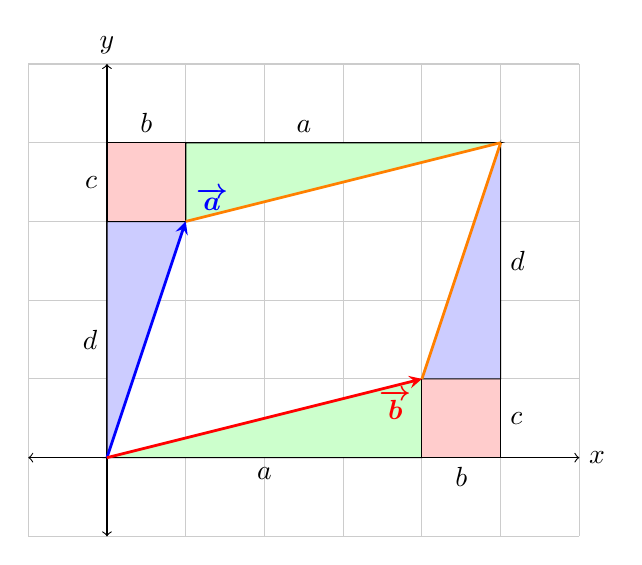
\begin{tikzpicture}
  \draw[thin,gray!40] (-1,-1) grid (6,5);
  \draw[<->] (-1,0)--(6,0) node[right]{$x$};
  \draw[<->] (0,-1)--(0,5) node[above]{$y$};
  
	\filldraw[fill=green!20] (0,0) node[anchor=north]{}
  -- (2,0) node[anchor=north]{$a$}
  -- (4,0) node[anchor=north]{}
  -- (4,1) node[anchor=south]{}
  -- cycle;
  
  	\filldraw[fill=red!20] (4,0) node[anchor=north]{}
  -- (4.5,0) node[anchor=north]{$b$}	
  -- (5,0) node[anchor=north]{}
  -- (5,0.5) node[anchor=west]{$c$}
  -- (5,1) node[anchor=south]{}
  -- (4,1) node[anchor=south]{}
  -- cycle;
  
  	\filldraw[fill=blue!20] (4,1) node[anchor=north]{}
  -- (5,1) node[anchor=north]{}
  -- (5,2.5) node[anchor=west]{$d$}
  -- (5,4) node[anchor=south]{}
  -- cycle;
  
  	\filldraw[fill=blue!20] (0,0) node[anchor=north]{}
  -- (0,1.5) node[anchor=east]{$d$}
  -- (0,3) node[anchor=north]{}
  -- (1,3) node[anchor=south]{}
  -- cycle;
  
	\filldraw[fill=red!20] (0,3) node[anchor=north]{}
  -- (0,3.5) node[anchor=east]{$c$}
  -- (0,4) node[anchor=north]{}
  -- (0.5,4) node[anchor=south]{$b$}
  -- (1,4) node[anchor=south]{}
  -- (1,3) node[anchor=south]{}
  -- cycle;
    
  	\filldraw[fill=green!20] (1,4) node[anchor=north]{}
  -- (2.5,4) node[anchor=south]{$a$}	
  -- (5,4) node[anchor=north]{}
  -- (1,3) node[anchor=south]{}
  -- cycle;
  
    \draw[line width=1pt,blue,-stealth](0,0)--(1,3) node[anchor=south west]{$\boldsymbol{\overrightarrow{a}}$};
  \draw[line width=1pt,red,-stealth](0,0)--(4,1) node[anchor=north east]{$\boldsymbol{\overrightarrow{b}}$};
  
  \draw[line width=1pt,orange](1,3)--(5,4) node[anchor=south west]{};
  \draw[line width=1pt,orange](4,1)--(5,4) node[anchor=north east]{};
	
	
\end{tikzpicture}

\begin{equation}
	det \bigg( \begin{bmatrix}
a & b\\\
c & d 
\end{bmatrix} \bigg) = (a+b) \cdot (d+c) - 2bc - db - ac = ad - bc
\end{equation}

\begin{equation} 
det \Bigg( \begin{bmatrix}
k_0 & v_0 & w_0 \\\
k_1 & v_1 & w_1 \\\
k_2 & v_2 & w_2
\end{bmatrix} \Bigg) = k_0 \cdot 	det \bigg( \begin{bmatrix}
v_1 & w_1\\\
v_2 & w_2 
\end{bmatrix} \bigg) - v_0 \cdot 	det \bigg( \begin{bmatrix}
k_1 & w_1\\\
k_2 & w_2 
\end{bmatrix} \bigg) + w_0 \cdot 	det \bigg( \begin{bmatrix}
k_1 & v_1\\\
k_2 & v_2 
\end{bmatrix} \bigg)
\end{equation}

\begin{equation} 
det \Bigg( \begin{bmatrix}
k_0 & v_0 & w_0 \\\
k_1 & v_1 & w_1 \\\
k_2 & v_2 & w_2
\end{bmatrix} \Bigg) = k_0 ( v_2 \cdot w_3 - v_3 \cdot w_2 ) + 
k_1 ( v_3 \cdot w_1 - v_1 \cdot w_3 )
+ k_2 (v_1 \cdot w_2 - v_2 \cdot w_1)
\end{equation}



\subsection*{ Scalar Produkt }

\begin{equation}
\overrightarrow{a} \cdot \overrightarrow{b} = \sum_{k=1}^n a_k \cdot b_k  = \vert \overrightarrow{a} \vert \cdot \vert \overrightarrow{b} \vert \cdot cos(\sphericalangle (\overrightarrow{a}, \overrightarrow{b} ))
\end{equation}
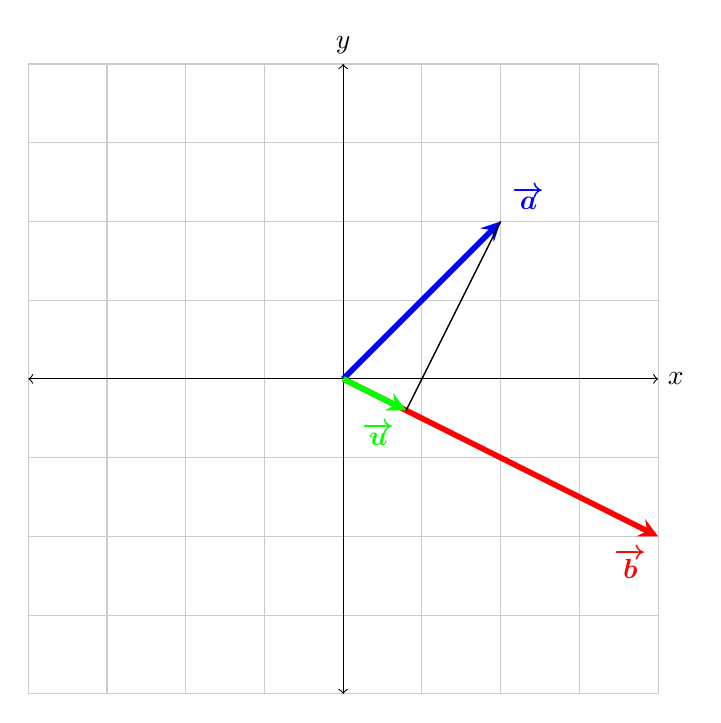
\begin{tikzpicture}
  \draw[thin,gray!40] (-4,-4) grid (4,4);
  \draw[<->] (-4,0)--(4,0) node[right]{$x$};
  \draw[<->] (0,-4)--(0,4) node[above]{$y$};
  \draw[line width=2pt,blue,-stealth](0,0)--(2,2) node[anchor=south west]{$\boldsymbol{\overrightarrow{a}}$};
  \draw[line width=2pt,red,-stealth](0,0)--(4,-2) node[anchor=north east]{$\boldsymbol{\overrightarrow{b}}$};
    \draw[line width=0.5pt,black](2,2)--(0.8,-0.4) node[anchor=north east]{};  
      \draw[line width=2pt,green,-stealth](0,0)--(0.8,-0.4) node[anchor=north east]{$\boldsymbol{\overrightarrow{u}}$};
  
\end{tikzpicture}

\( \overrightarrow{a} \cdot \overrightarrow{b} = \vert \overrightarrow{u} \vert \cdot \vert \overrightarrow{b} \vert \Rightarrow \vert \overrightarrow{u} \vert =  cos(\sphericalangle (\overrightarrow{a}, \overrightarrow{b} )) \cdot \vert \overrightarrow{a} \vert \)

Wobei \( \overrightarrow{b} \) Immer der Vektor ist auf dem \( \overrightarrow{u} \) Projeziert wird. \newline 

Das Dot Product kann aber auch als ein Matrix Vector produkt verstanden werden wobei die Lineare Abbildung alles auf eine Achse zusammen presst. Somit ist diese Matrix immer eine \( ( 1 \times n ) \) Matrix weil wir zu Faul sind die Nullen mit zuschreiben.

\begin{equation} 
\begin{bmatrix}
\ihat_0 & \jhat_0
\end{bmatrix}  
\cdot 
\begin{pmatrix}
x_1 \\ x_2
\end{pmatrix} = \ihat_0 \cdot x_1 + \jhat_0 \cdot x_2 
\end{equation}


Note für Verständniss: \( \begin{bmatrix}
\ihat_0 & \jhat_0
\end{bmatrix}   \) Kann hier als Rotierte Achse Verstanden werden die Anderen Vektoren wird auf diese Achse Projeziert.

\subsection*{ Kreuz Produkt} 

\subsubsection*{ In 2 Dimensions}

\begin{equation}
	 \begin{pmatrix}
	 	a  \\\
	 	b
	 \end{pmatrix} \times 	 \begin{pmatrix}
	 	c  \\\
	 	d
	 \end{pmatrix} = det \bigg( \begin{bmatrix}
	 	a & c \\\
	 	b & d
	 \end{bmatrix} \bigg) = a \cdot c - b \cdot d
\end{equation}

\subsubsection*{In 3 Dimensions }

In \( n = 3 \) Dimensionen .
\( \overrightarrow{a} \times \overrightarrow{b} = \begin{pmatrix}
	a_3 \cdot b_2 - a_2 \cdot b_3 \\ a_1 \cdot b_3 - a_3 \cdot b_1 \\ a_2 \cdot b_1 - a_1 \cdot b_2
\end{pmatrix} \) 

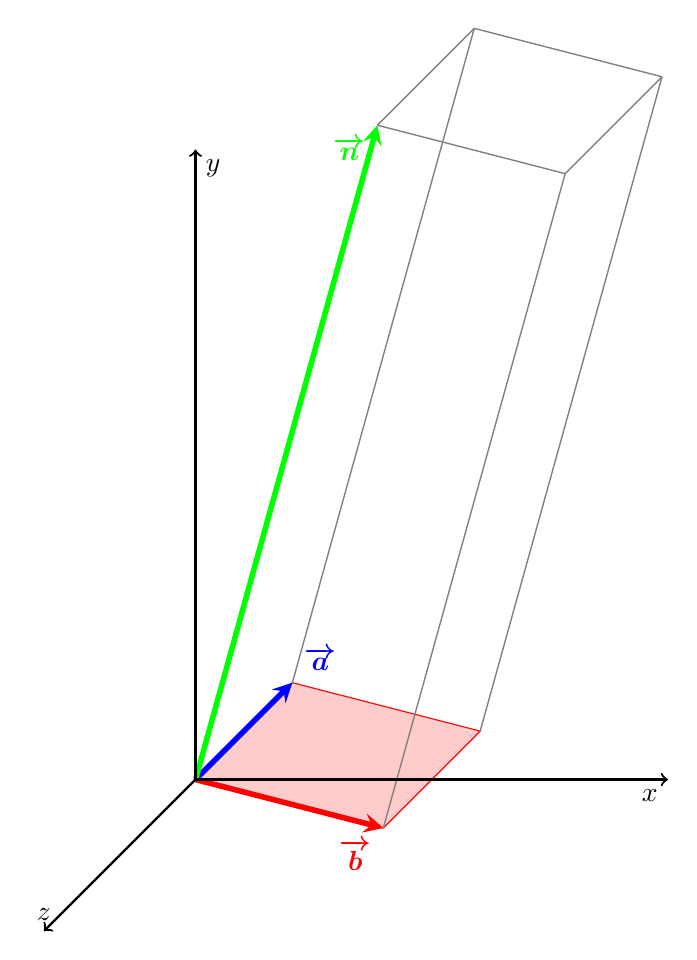
\begin{tikzpicture}[scale=1]

	    
    
    \def\x{.5}
    \filldraw[
        draw=red,%
        fill=red!20,%
    ]          (0,0,0)
            -- (2,2,2)
            -- (4,1,1)
            -- (2,-1,-1)
            -- cycle;
            
	\draw[line width=2pt,blue,-stealth](0,0,0)--(2,2,2) node[anchor=south west]{$\boldsymbol{\overrightarrow{a}}$};
  	\draw[line width=2pt,red,-stealth](0,0,0)--(2,-1,-1) node[anchor=north east]{$\boldsymbol{\overrightarrow{b}}$};
	\draw[line width=2pt,green,-stealth](0,0,0)--(0,6,-6) node[anchor=north east]{$\boldsymbol{\overrightarrow{n}}$};
	
	\draw[line width=0.5pt,gray](2,2,2)--(2,8,-4) node[anchor=north east]{};
	
	\draw[line width=0.5pt,gray](2,-1,-1)--(2,5,-7) node[anchor=north east]{};
	
	\draw[line width=0.5pt,gray](4,1,1)--(4,7,-5) node[anchor=north east]{};
	\draw[line width=0.5pt,gray](0,6,-6)--(2,8,-4) node[anchor=north east]{};
	\draw[line width=0.5pt,gray](2,8,-4)--(4,7,-5) node[anchor=north east]{};
	\draw[line width=0.5pt,gray](4,7,-5)--(2,5,-7) node[anchor=north east]{};
	\draw[line width=0.5pt,gray](2,5,-7)--(0,6,-6) node[anchor=north east]{};	
	\draw[thick,->] (0,0,0) -- (6,0,0) node[anchor=north east]{$x$};
	\draw[thick,->] (0,0,0) -- (0,8,0) node[anchor=north west]{$y$};
    \draw[thick,->] (0,0,0) -- (0,0,5) node[anchor=south]{$z$};
\end{tikzpicture}

Für die Herleitung das Spatprodukt ist gleich der Determinante der \( ( 3 \times 3 ) \) Matrix aus dem 3. Vektor des Spat Produkt und den beiden Richtungsvektoren \( \overrightarrow{a} \land \overrightarrow{b} \)

\begin{equation}
	\begin{pmatrix}
		 p_1 \\\ p_2 \\\ p_3
	\end{pmatrix} \cdot \begin{pmatrix}
		 x \\\ y \\\ z
	\end{pmatrix} = det \Bigg( \begin{bmatrix}
		x & v_1 & w_1 \\\
		y & v_2 & w_2 \\\
		z & v_3 & w_3 
	\end{bmatrix} \Bigg)
\end{equation}

\begin{equation}
	p_1 \cdot x + p_2 \cdot y + p_3 \cdot z = x ( v_2 \cdot w_3 - v_3 \cdot w_2 ) + 
y ( v_3 \cdot w_1 - v_1 \cdot w_3 )
+ z (v_1 \cdot w_2 - v_2 \cdot w_1)
\end{equation}

\begin{equation}
\overrightarrow{p} = \begin{pmatrix}
v_2 \cdot w_3 - v_3 \cdot w_2 \\\
v_3 \cdot w_1 - v_1 \cdot w_3 \\\
v_1 \cdot w_2 - v_2 \cdot w_1
\end{pmatrix}
\end{equation}

Der Flächeninhalt der von \( \overrightarrow{a} \land  \overrightarrow{b} \) eingeschlossenen Fläche ist \( \vert \overrightarrow{a} \times \overrightarrow{b} \vert \)

\subsection*{ Spatprodukt }

\( (\overrightarrow{a} \times \overrightarrow{b}) \cdot \overrightarrow{c} = V \)

\subsection*{ Punkt Ebene Beziehung }

\( 0 = \overrightarrow{n} \cdot (\overrightarrow{x}- \overrightarrow{p}) \land \overrightarrow{x} = \overrightarrow{r} + t \cdot \overrightarrow{n}  \land \overrightarrow{RF} = t \cdot \overrightarrow{n} \land \vert \overrightarrow{RF} \vert = d \)
Gerade in die Ebene einsetzten und nach der Laufvariable der geraden t umstellen ergibt. \( t = \frac{ \overrightarrow{n} \cdot ( \overrightarrow{p} - \overrightarrow{r}) }{ \vert \overrightarrow{n} \vert ^2} \) Wenn wir das jetzt in \( d = \vert t \cdot \overrightarrow{n } \vert \) einsetzen erhalten wir: \( d = \frac{\vert \overrightarrow{n} \cdot ( \overrightarrow{p} - \overrightarrow{r} ) \vert }{\vert \overrightarrow{n} \vert } \) ähnelt der Hesschen Normal Form \( \Rightarrow d = \vert \overrightarrow{n_0} \cdot ( \overrightarrow{r} - \overrightarrow{p} ) \vert \) Das absolut weil ein Abstand immer positiv ist.

\subsection*{ Lagebeziehungs Verschiedener Objekte } 

Windschief: \( g_1 \cap g_2 = \emptyset \land \text{linear unabhängig} \)


\paragraph*{ Gerade - Gerade } (Windschief , \( \parallel \), \( \equiv \), \( g_1 \cap g_2 = S \))

\paragraph*{ Gerade - Ebene} (\( \parallel \),\( \equiv \), \( g \in \varepsilon \), \( g \cap \varepsilon = S \))

\paragraph*{ Ebene - Ebene} (\( \parallel \), \( \equiv \), \( \varepsilon_1 \cap \varepsilon_2 = g \))

\subsubsection*{ Coole Ideen die ich mir Merken sollte}

Der Richtungs Vektor der Schnittgeraden zweier Ebenen ist das Kreuzprodukt der Beiden Normal Vektoren. \newline

Richtungs Vektor einer Geraden als Normalen Vektoren einer Ebene betrachten für Berechnungen wie min Abstand zweier Windschiefer geraden.


\end{document}